\documentclass{standalone}
\usepackage{tikz}
\begin{document}
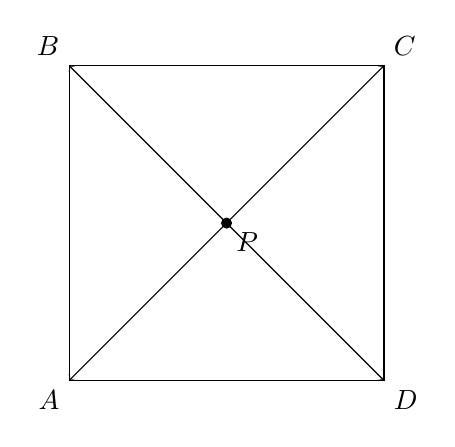
\begin{tikzpicture}
  \draw (0,0) rectangle (4,4); % Draw the square
  \fill (2,2) circle[radius=2pt]; % Draw the center point
  \draw[->] (2,2) -- (0,0); % Draw the first line
  \draw[->] (2,2) -- (0,4); % Draw the second line
  \draw[->] (2,2) -- (4,4); % Draw the third line
  \draw[->] (2,2) -- (4,0); % Draw the fourth line
  \node at (2,2) [below right] {$P$}; % Label the center point
  \node at (0,0) [below left] {$A$}; % Label the first corner
  \node at (0,4) [above left] {$B$}; % Label the second corner
  \node at (4,4) [above right] {$C$}; % Label the third corner
  \node at (4,0) [below right] {$D$}; % Label the fourth corner
\end{tikzpicture}
\end{document}
